\documentclass[a4paper, 11pt]{article}
\def\AssTeX{ % "A Magnum Opus of LaTeX shitposting." -IGN, 9.5/10
	A\kern-.36em
	{\setbox0=\hbox{T}%
	 \vbox to \ht0{\hbox{\the\scriptfont0 SS}\vss}}%
	\kern-.15em
	\TeX
}
\usepackage[T1]{fontenc} % 
\usepackage{lmodern} % Roman type %% \usepackage{tgpagella}
\usepackage[scaled=0.8]{beramono} % Mono type for lmodern %% \usepackage[scaled=0.8]{roboto-mono},
%\usepackage{helvet} % Sans type
%	\renewcommand{\familydefault}{\sfdefault}
%\usepackage[scaled=0.85]{beramono} % Mono type for helvet
\usepackage[top=3.5cm, bottom=3.5cm, left=3.5cm, right=3.5cm]{geometry} % Page geometry
%\usepackage{parskip} % No paragraph indent
	\setlength{\parindent}{0pt} % Have no indent
	%\setlength{\parskip}{1.2ex} % Have vertical space
\usepackage{fancyhdr} % Custom page header
	\pagestyle{fancy} \fancyhf{} \headheight 26pt
	\renewcommand{\sectionmark}[1]{\markright{#1}{}}
	\lhead{\large An Assemblage of Typesetting Examples}
	 \chead{}
	  \rhead{\rightmark}
	\lfoot{\textcolor{textcol!5!pagecol}{\quad$\mathcal{L}$.}}
	 \cfoot{}
	  \rfoot{\small\thepage\ of \pageref{LastPage}}
\usepackage{amsmath,amssymb,stmaryrd} % Math and symbols %% \lightning
	\def\N{\mathbb{N}} % Natural numbers %% \N
	\def\R{\mathbb{R}} % Real numbers %% \R
	\def\C{\mathbb{C}} % Complex numbers %% \C
	\def\HT{\mathsf{H}} % Hermitian transpose %% \HT
	\def\On{\mathcal{O}} % O-notation %% \On
	\def\de{\mathrm{d}} % Derivative %% \de
	\DeclareMathOperator{\id}{id} % Identity
\usepackage{centernot,mleftright} % Extra formatting %% \centernot{symbol} %% \mleft( \mright)
	\newcommand{\floor}[1]{{\left\lfloor{#1}\right\rfloor}} %% \floor{expression}
	\newcommand{\ceil}[1]{{\left\lceil{#1}\right\rceil}} %% \ceil{expression}
	\newcommand{\norm}[1]{{\left\|{#1}\right\|}} %% \norm{expression}
	\newcommand{\angles}[1]{{\left\langle{#1}\right\rangle}} % \angles{expression}
\usepackage[rgb]{xcolor} % Colorful text
	\definecolor{wikiblue}{HTML}{3366CC}
	\definecolor{discordred}{HTML}{ED4245}
	\definecolor{blurple}{HTML}{5865F2}
	\definecolor{vigor}{HTML}{35D7BB}
	\definecolorseries{BLU}{hsb}{step}[HTML]{008CFF}{0,-.01,0} \resetcolorseries[100]{BLU}
		\colorlet{brandblue}{BLU!![35]}%\definecolor{brandblue}{HTML}{57B2FF}
		\colorlet{grayblue}{BLU!![70]!70!black}%\definecolor{grayblue}{HTML}{7C98AB}
		\colorlet{graymoss}{grayblue>wheel,11,12}
	\definecolor{pergament}{HTML}{EFE2CF}%{FAF0C8}%\definecolor{pergament}{RGB}{239,234,210}
	\definecolor{sepia}{HTML}{322D23}%{271E17}
	\definecolor{dark}{HTML}{36393F}
	\definecolor{light}{HTML}{DCDDDE}
	\providecolor{pagecol}{named}{white} \pagecolor{pagecol}
	\providecolor{textcol}{named}{black} \color{textcol}
\usepackage{tikz} % TikZ ist ein Zeichenprogramm
\usepackage{pgfplots} % Plot graphs
	\pgfplotsset{compat=1.18}
\usepackage{graphicx} % Graphics formatting
	\graphicspath{{resources/}}
	\newcommand{\emoji}[1]{\raisebox{-0.4ex}{\includegraphics[height=2.5ex]{#1}}} %% \emoji{name}
\usepackage{float} % Float placement %% [H]
\usepackage{wrapfig} % Wrapping figures
\usepackage{caption} % To prevent "Figure #: "
\usepackage{subcaption} % Several figures side-by-side
\usepackage{hyperref} % Hyperlinks
	\hypersetup{colorlinks=true, urlcolor=wikiblue, linkcolor=blue}%allcolors
\usepackage[most]{tcolorbox} % Nice colorboxes
	\newtcolorbox{mybox}[2]{ %% \begin{mybox}{color}{additional_box_parameters} stuff \end{mybox}
	    enhanced, breakable,
	    fonttitle=\sffamily\small\bfseries, fontupper=\normalsize,
	    boxrule=0.35mm, arc=1mm,%arc is angular,
	    sharp corners=downhill,
	    colframe=#1,
	    coltitle=pagecol, coltext=textcol,
	    colbacktitle=#1!80!pagecol, colback=#1!10!pagecol,
	    #2
	}
	\newcommand{\lthm}[1]{ %% \lthm{theorem}
		\begin{mybox}{brandblue}{title=Theorem,
			attach boxed title to top left={yshift=-0.35mm,},
	    	boxed title style={
	    		boxrule=0.35mm, arc=1mm,%arc is angular,
	    		sharp corners=all, rounded corners=northeast,
	    	},
	    }
			{#1}
		\end{mybox}
	}
	\newcommand{\ldef}[2]{ %% \ldef{definition_name}{definition}
		\begin{mybox}{grayblue}{adjusted title={Definition: {#1}}}
			{#2}
		\end{mybox}
	}
	\newcommand{\lsubdef}[1]{\tcbsubtitle[top=0.6mm]{Definition: {#1}}} %% \lsubdef{definition_name}
\usepackage{listings} % Code listing
	\lstdefinelanguage{customlang}{morecomment=[l]{//}, morekeywords={if,else,while,for,return}}
	\lstdefinestyle{L}{ %% \begin{lstlisting}[style=L] stuff \end{lstlisting}
		language=customlang, mathescape=true,
		xleftmargin=0.05\textwidth, xrightmargin=0.05\textwidth,%frame=tblr,
    	basicstyle=\ttfamily,%\small,
    	keywordstyle=\bfseries,
    	commentstyle=\color{textcol!50!pagecol}\itshape, 
    	numberstyle=\ttfamily\color{textcol!75!pagecol}\scriptsize,          
    	numbers=left,%numbersep=3mm,
    	breaklines=true, tabsize=4, keepspaces=true, showstringspaces=false,
	}
	\lstset{style=L}
	\newenvironment{lalg}[1]{ %% \begin{lalg}{algorithm_name} stuff \end{lalg}
		\begin{mybox}{graymoss}{adjusted title={Algorithm: {#1}}}
	}{
		\end{mybox}
	}
%	\DeclareTCBListing{codebox}{ !O{} }{ %% \begin{codebox}[optional_title] your_code \end{codebox}
%        enhanced, breakable,
%        boxrule=0.35mm, arc=0mm,%arc is angular,sharp corners=downhill,
%        colframe=blurple!50!pagecol, colbacktitle=blurple!35!pagecol, colback=blurple!7!pagecol,
%        listing options={}, listing only,
%        title={#1}, toptitle=0.5mm, bottomtitle=0.3mm,
%    }
\usepackage{needspace} % Keep two paragraphs from detaching
	\newcommand{\exercise}[1]{ %% \exercise{number}
		\bigskip\par\noindent\needspace{2\baselineskip}
		\textbf{\large Exercise #1.}\quad
	}
\usepackage{enumitem} % Custom enumeration
	\newenvironment{subtasks}{ %% \begin{subtasks} stuff \end{subtasks}
		\begin{enumerate}[label=\alph*)]
	}{
		\end{enumerate}
	}
\usepackage{bookmark} % Digital bookmarks
	\newcommand{\week}[1]{%
		\par\noindent\centerline{%
			\color{textcol!50!pagecol}%
			\texttt{\footnotesize #1\space}%
			\rule{1\textwidth}{0.35mm}%
		}%
		\bookmark[page=\thepage]{Notes #1}%
	} %% \week{number}
\usepackage{multicol} % Multiple page columns
\usepackage[normalem]{ulem} % Fancier underlining %% \sout{text}, \dotuline{text} 
\usepackage{shapepar} % Paragraph shapes
\usepackage{tabularx,booktabs} % Better tables
	\newcolumntype{Y}{>{\centering\arraybackslash}X}
\usepackage{multirow} % Span multiple rows in a table
\usepackage{moreverb} % Better verbatim environment
\usepackage[nottoc]{tocbibind} % Add bibliography and list of X to toc
%\usepackage[backend=biber, style=alphabetic, sorting=ynt]{biblatex} % Bibliographies - https://tex.stackexchange.com/questions/63852/question-mark-or-bold-citation-key-instead-of-citation-number
%	\addbibresource{resources/references.bib}
%\usepackage{natbib} % Bibliography - https://www.overleaf.com/learn/latex/Bibliography_management_with_natbib
%	\bibliographystyle{plain}
\usepackage{eso-pic} % Insert images behind text
\usepackage{rotating} % Rotat e
\usepackage{afterpage} % Reset page color
\usepackage{lastpage} % Reference last document page
%\usepackage{manfnt} % \dbend
\usepackage{scrextend} % Change margins(indent) selectively
	\newcommand{\todo}{ %% \todo
		\scalebox{0.8}[1.0]{
			\fcolorbox{discordred}{brandblue!10!pagecol>wheel,1,2}{
				\color{discordred}
				\textsc{\small todo}
			}
		}
	}
	\newcommand{\toco}{ %% \toco
		\scalebox{0.6}[0.75]{
			\fcolorbox{vigor}{vigor!10!pagecol>wheel,10,12}{
				\color{vigor}
				\textsc{\small toco}
			}
		}
	}
\usepackage{bussproofs} % Proof trees
	\newcommand{\unary}[1]{\UnaryInfC{#1}} %% \unary{stuff}
	\newcommand{\binary}[1]{\BinaryInfC{#1}} %% \binary{stuff}
	\newcommand{\ternary}[1]{\TrinaryInfC{#1}} %% \ternary{stuff}
	\newcommand{\rulename}[1]{\RightLabel{\scriptsize #1}} %% \rulename{name_of_rule}
	\def\axiom{\AxiomC{} \rulename{Ax}} %% \axiom
	\def\seq{\;\vdash\,} % Syntactic entailment symbol %% \seq
\includeonly{
	main_templates,
	main_text,
	main_mathematics,
	main_tables,
	main_images,
	main_drawing,
	main_random,
	main_bibliography,
}

% ~:------------------------------------+------------------------------------:~

                                 \begin{document}

% ~:------------------------------------+------------------------------------:~

% Cover page
\begingroup
	\pagecolor[HTML]{4A4951}
	\thispagestyle{empty}
	\AddToShipoutPicture*{
		\put(-4,0){
			\parbox[b][\paperheight]{\paperwidth}{
				\vfill
%				\centering
				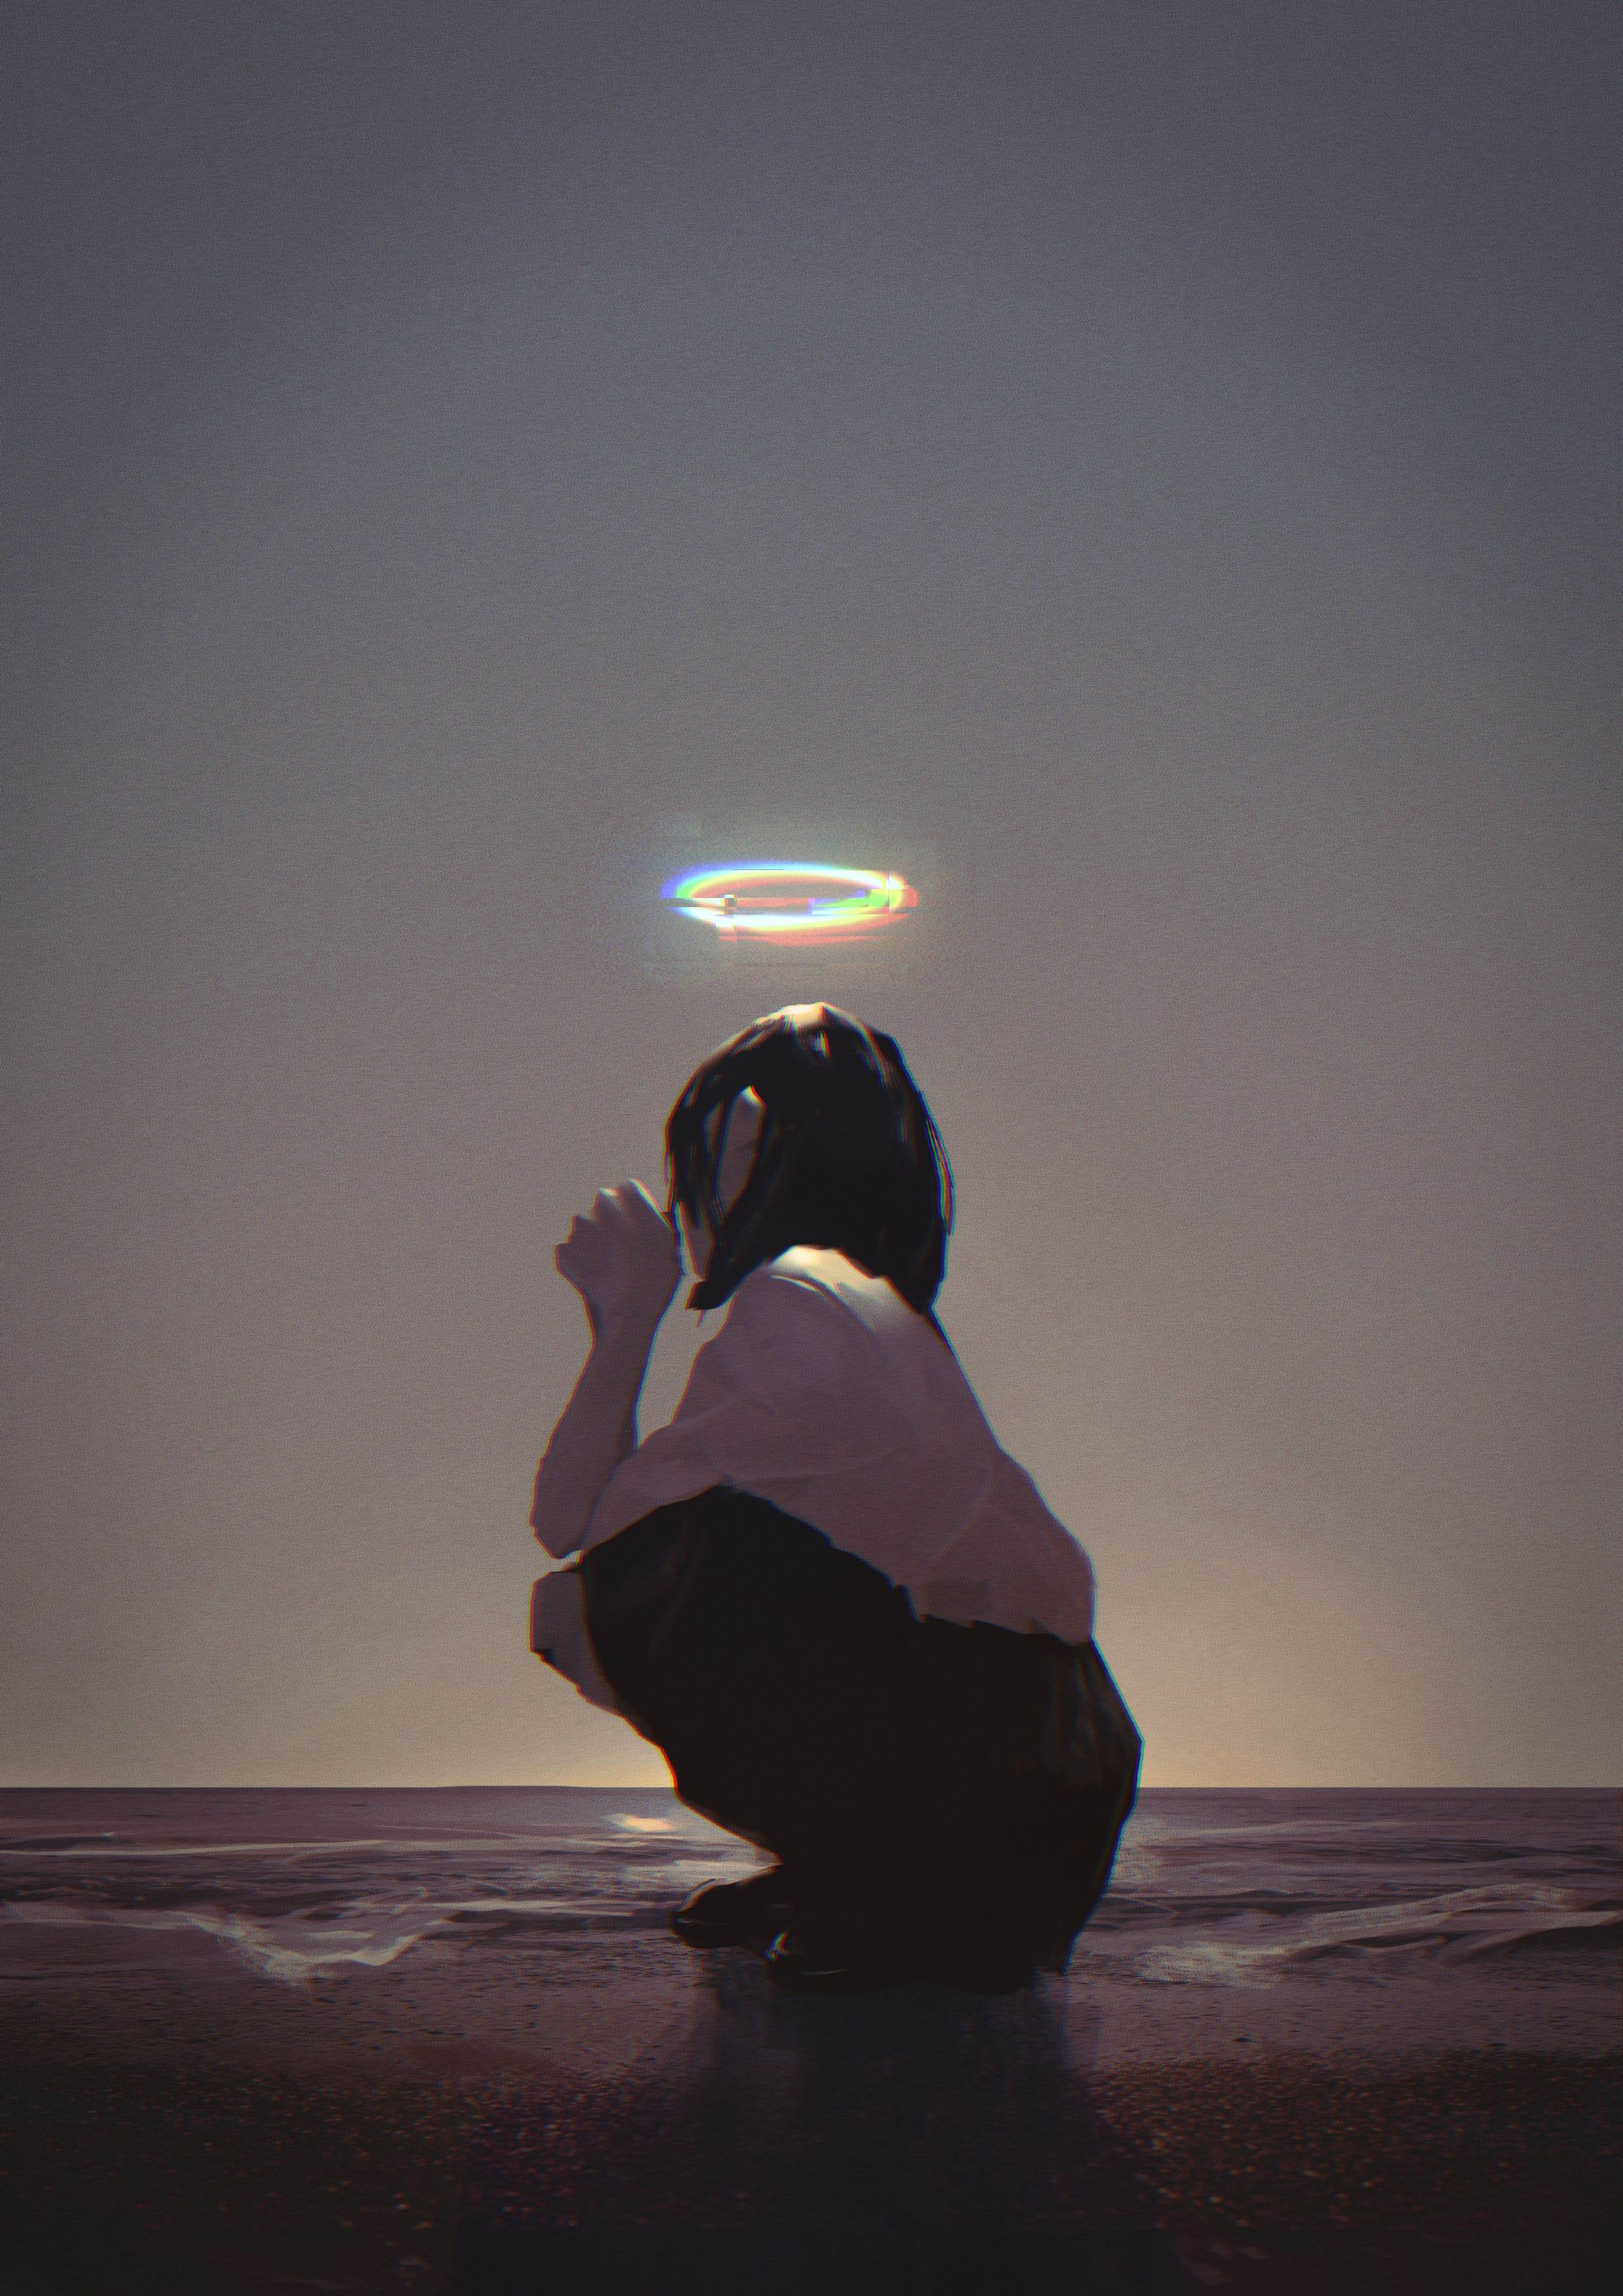
\includegraphics[width=1\paperwidth]{resources/background.jpg}
				\vfill
			}
		}
	}
	\begin{figure}[H]
		\centering
%		\vspace*{0.1\paperheight}
		\vspace*{0.03\paperheight}
		\color{pergament}
		\textsc{
			\Huge
			An Assemblage of \\
			Typesetting Examples \\
		}
%		\vspace*{0.55\paperheight}
		\href{https://www.pixiv.net/en/artworks/93550054}{\textsc{\tiny\color[HTML]{56555D}Image by Neg}}
	\end{figure}
	\afterpage{\pagecolor{pagecol}}
	\clearpage
	\addtocounter{page}{-1}
\endgroup

% Store title information
\title{An Assemblage of Typesetting Examples}
\author{George P. Burdell \& Chris P. Bacon \& Lucas W.\thanks{It would not have been possible to finish \textsc{An Assemblage of Typesetting Examples} a.k.a.{} \AssTeX{} without the \scalebox{1.2}[1.0]{unrelenting} support of F.D.C. Willard and Sleve McDichael. Many thanks!}}
\date{\today}
% This allows us to sneak in stuff before a title
{\textcolor{textcol!5!pagecol}{\hfill\tiny riverrun}\let\newpage\relax
% Print the title
\maketitle }
% Change name of an abtract before writing it
\renewcommand{\abstractname}{AbstReAct}
\begin{abstract}
	Cubum autem in duos cubos, aut quadratoquadratum in duos quadratoquadratos et generaliter nullam in infinitum ultra quadratum potestatem in duos eiusdem nominis fas est dividere cuius rei demonstrationem mirabilem sane detexi. Hanc marginis exiguitas non caperet. % https://en.wikipedia.org/wiki/Fermat%27s_Last_Theorem
\end{abstract}
\begin{center}
	\small
	\textit{``A Magnum Opus of \LaTeX{} tomfoolery.''}%\href{https://en.wikipedia.org/wiki/Shitposting}{\color{textcol}sh\!$\mathrel{\ooalign{\hss$\circ$\hss\cr$\times$}}$\!tposting}.''}
	-- $\mathfrak{The\ Authentic\ Newspaper}$
	
	\medskip
	Compiled with Lua\LaTeX{}.
\end{center}
% Print autogenerated table of contents
\tableofcontents
% Remove page number
\thispagestyle{empty}
% Finish this page manually	
\clearpage

% Demonstrate including a file - https://www.overleaf.com/learn/latex/Management_in_a_large_project
% Note the difference it has opposed to plain input - https://tex.stackexchange.com/questions/246/when-should-i-use-input-vs-include
% Start an unnumbered section and add it to the table of contents manually
\section*{0. Custom Templates}
\addcontentsline{toc}{section}{Custom stuff}

% Start a subsection
\subsection{Lecture notes template}

\subsubsection{Weekly notes}

% Insert week marker and separator
\week{1}

% Use custom command defined in preamble to add a 'definition' box
\ldef{Träger}{
	Sei $f:\R\to\R$ stetig.
	Der Träger von $f$ (support) ist
		\[ \{x\in\R \mid f(x)\neq 0\} = \operatorname{supp}(f) \]
	Die Fkt. $f$ hat kompakten Träger genau dann wenn $f(x) = 0$ $\forall x\in\R$ mit $|x|>R$,	für ein $R>0$ gross genug.
% Add another 'definition' inside same box
	\lsubdef{Faltung}
	Sei $f:\R\to\R$ stetig, und sei $\psi:\R\to\R$ stetig mit kompaktem Träger.
	Die Faltung von $f$ mit $\psi$ (convolution) ist die Funktion $\psi*f:\R\to\R$,
		\[ (\psi*f)(x) = \int_{-\infty}^{+\infty} \psi(x-y)f(y) \,\de y \]
}

\week{69}

% Add a 'theorem' box
\lthm{
	Let $S$, $T$ be statements.
	Let "$\overset.\implies$" be the (informal) \textit{triviality} relation, i.e. $S\overset.\implies T$ if and only if $T$ is trivially provable from $S$.
	Then triviality ("$\overset.\implies$") is not transitive.
}

\subsection{Exercise sheet template}

% Add an 'exercise' title
\exercise{42} \textit{Prove the theorem given above.}
% Begin enumerating subtasks
\begin{subtasks}
	\item I saw Fermat in the elevator and he said he had a \href{https://ocw.mit.edu/courses/6-042j-mathematics-for-computer-science-fall-2010/9f565760fc876e8ce22f822e7471faa9_MIT6_042JF10_proof.pdf}{proof}\dots
    \item This exercise is left as a proof to the teaching assistant.
\end{subtasks}

\section{Text Stuff}
% Demonstrate that spurious whitespace and comments are ignored
The following  itemized   list
demonstrates
    some standard 
%
text
%
%
    formatting options.

% Format a list in two columns
\begin{multicols}{2}
% Format an itemized list
% Optionally specify spacing between items
\begin{itemize}[itemsep=0mm]
% Use custom label for one item
	\item[\checkmark] Normal text.
% Demonstrate text formatting commands
	\item \textrm{Serif text.}
	\item \textbf{Bold text.} % ≈ {\bfseries text}
	\item \textit{Italic text.} % ≈ {\itshape text}
	\item \textbf{\textit{Bold Italic text.}}
	\item \textsc{Small caps.}
	\item \textsf{Sans serif text.} % ≈ {\sffamily text}
	\item \texttt{Typewriter text.} % ≈ {\ttfamily text}
	\item \textsl{Slanted text.}
	\item[\vspace{\fill}] % Fill list to guarantee same spacing in second column
\end{itemize}
\end{multicols}

% Demonstrate formatting of URLs and links
URLs look like this: \url{https://oeis.org/wiki/List_of_LaTeX_mathematical_symbols}.
Otherwise \href{http://jwilson.coe.uga.edu/EMT668/EMAT6680.F99/Challen/proof/proof.html}{hyperlinks} are also possible.
% Demonstrate footnotes and margin notes
Footnotes can be done like this\footnote{hello, world} and \dotuline{margin notes}\reversemarginpar\marginpar{\raggedleft\footnotesize 'Tis a left-sided margin note to admire.} similarly so.
% Demonstrate refs
In the same vein we can easily make references to figures, tables, equations and sections (e.g. for more formatting refer to section \ref{sec:tables} containing table \ref{tab:sizes} on page \pageref{tab:sizes} which specifies text and math font size commands).
% Demonstrate hyperlinks
% -> `\hypertarget{...}`
But generally it is possible to link directly to any word or sentence in your \hyperlink{thelink}{document.}
% Demonstrate references
References to outside sources are citations, e.g., ``\LaTeX{} \cite{lamport94} is a set of macros built atop \TeX{} \cite{texbook}.''

We enumerate some customisation options useful in edge cases:
% Demonstrate enumeration
\begin{enumerate}
	\item \verb`spa~ce` inserts an unbreakable space in 'spa~ce', whereas \verb`wo\-rd` allows 'wo\-rd' to be broken.
% This is an ad-hoc macro
	\def\mgn{-.08ex}
	\item Raise or lower the vertical position of \raisebox{\mgn}{indi\raisebox{\mgn}{vid\raisebox{\mgn}{ua\raisebox{\mgn}{\raisebox{\mgn}{l t\raisebox{\mgn}{\raisebox{\mgn}{hi\raisebox{\mgn}{\raisebox{\mgn}{n\raisebox{\mgn}{\raisebox{\mgn}{g\raisebox{\mgn}{\raisebox{\mgn}{\raisebox{\mgn}{s}.}.}}.}}}.}}}.}}.}.}..
	\item Do manu\kern0.15em al ker\kern-.15em ning (kerning)
	\item Scale things in \scalebox{1.25}[0.75]{either} \scalebox{0.67}[1.33]{dimension} or change both axes:
% Demonstrate heart-shaped paragraph being wrapped in a minipage of certain size that can be more easily rescaled
	\resizebox{!}{25pt}{\begin{minipage}{\textwidth}\heartpar{Number 15: Burger king foot lettuce. The last thing you'd want in your Burger King burger is someone's foot fungus. But as it turns out, that might be what you get. A 4channer uploaded a photo - anonymously - to the site, showcasing his feet in a plastic bin of lettuce, with the statement: "This is the lettuce you eat at Burger King." Admittedly, he had shoes on. But that's even worse. The post went live at 11:38 PM on July 16, and a mere 20 minutes later, the Burger King in question was alerted to the rogue employee. At least, I hope he's rogue. How did it happen? Well, the BK employee hadn't removed the Exif data from the uploaded photo, which suggested the culprit was somewhere in Mayfield Heights, Ohio. This was at 11:47. Three minutes later at 11:50, the Burger King branch address was posted with wishes of happy unemployment. 5 minutes later, the news station was contacted by another 4channer. And three minutes later, at 11:58, a link was posted: BK's "Tell us about us" online forum. The foot photo, otherwise known as exhibit A, was attached. Cleveland Scene Magazine contacted the BK in question the next day. When questioned, the breakfast shift manager said "Oh, I know who that is. He's getting fired." Mystery solved, by 4chan. Now we can all go back to eating our fast food in peace.}\end{minipage}}
\end{enumerate}

% Demonstrate verbatim
% Demonstrate crude framed box `\fbox` - https://en.wikibooks.org/wiki/LaTeX/Boxes
Further, use \verb`\verb#text#` -- '\texttt{\#}' being a delimiter of choice -- to display {\LaTeX} commands - including all special characters \fbox{\textbackslash\{\}\_\^{}\#\&\$\%\~{}} - and print them verbatim\renewcommand{\thefootnote}{$\star$}\footnote{Another footnote remarking on the fact that \texttt{\textbackslash verb} \sout{ironically} broke in an attempt of using it in a footnote $\overset\shortparallel\frown$}: \verb`\{}_^#&$%~`.

\medskip
\textcolor[HTML]{FF7F7F}{Naturally,}
\textcolor[HTML]{FFBF7F}{text}
\textcolor[HTML]{BFFF7F}{can}
\textcolor[HTML]{7FFFBF}{be}
\textcolor[HTML]{7FBFFF}{colored}
\textcolor[HTML]{BF7FFF}{in}
\textcolor[HTML]{FF7FBF}{as}
\textcolor[HTML]{FF7F7F}{well.}

\textcolor{-pagecol}{Mixing} colors is \textcolor{yellow!75!red}{easy!}

\textcolor{BLU!![0]}{Making}
\textcolor{BLU!![12]}{variations}
\textcolor{BLU!![25]}{in}
\textcolor{BLU!![37]}{saturation}
\textcolor{BLU!![50]}{is}
\textcolor{BLU!![62]}{a}
\textcolor{BLU!![75]}{little}
\textcolor{BLU!![87]}{more}
\colorbox{pagecol!75!black}{
	\textcolor{BLU!![100]}{involved.}
}%\footnote{Idea: spoilers could be done \colorbox{black}{\color{black}this?}}

% Diamond paragraph
\begin{figure}
	\hypertarget{thelink}{}
	\color{cyan!50!blue!80!black!75!white}
	\diamondpar{this song is actually about a grasshopper who doesn't spend enough time with his family because of work, and he wears a hat and carries a suitcase and everything, it's like Kafka, \color{cyan!50!blue!80!black!75!black}but then he has a change of heart and we see images of him and his lovely wife and children doing something together, like gardening or some shit}
	\captionsetup{font=tiny}
	\caption*{\href{https://www.newgrounds.com/audio/listen/522338}{OcularNebula, Forest of Fog}}
	\label{fig:diamond}
\end{figure}

\medskip
Selectively adapt margins, like this explanation of 
\\ \lstinline[language=Haskell]{data Parser a  =  String -> [(a, String)]}:
\vfill
\begin{addmargin}[2cm]{1cm}
	A parser for things \\
	is a function from strings \\
	to lists of pairs \\
	of things and strings
\end{addmargin}
\vfill

%稲葉曇『ラグトレイン』Vo. 歌愛ユキ % The day I can simply write stuff like this and it just *displays correctly* is gonna be remaRKABLE!!!!!

\section{Math Stuff}

% Demonstrate inline math - https://www.overleaf.com/learn/latex/Mathematical_expressions
% $i$ or \(i\)
Inline math allows us to state $e^{i\pi} + 1 = 0$ without interruption.
Display math is useful for important equations etc., which may in some cases requires bigger notation, such as matrices and case distinctions.
% Demonstrate display math
% \[ D \] preferable to $$ D $$
\[
	1
	= \det I_n
% Parenthesized matrix - https://www.overleaf.com/learn/latex/Matrices
	= \det\begin{pmatrix}
	1      & 0 & \cdots & 0      \\
	0      & 1 &        & 0      \\
	\vdots &   & \ddots & \vdots \\
	0      & 0 & \cdots & 1      \\
	\end{pmatrix}
% Custom bracket size
% Overbraces with `\overbrace{x}^{y}`
% Text in math with `\text` and nested math with $$
% Stacking symbols with `\stackrel`
% Case distinctions with `\begin{cases}`
	= \det\Big|\overbrace{ (\delta_{ij})_{ij} }^{\in\C^{n\times n}}\Big|
	\quad\text{where}\ \delta_{ij}
	:= \begin{cases} % https://math.stackexchange.com/questions/944757/whats-the-most-right-symbol-to-use-for-defined-to-be-equal-to
		1 & \text{if $i = j$} \\ 0 & \text{else.}
	\end{cases}
\]

We can refer to labeled equations, such as equation \eqref{eq:1}.

\textit{Given $\delta(P) = \max_{1\leq i\leq n}\{x_i-x_{i-1}\}$ for some partition $P = \{x_0,\dots,x_n\}\subseteq I$.
The function $f:I\to\R$ is integrable iff the following limit exists:}
% Demonstrate a math equation
\begin{equation}\label{eq:1}
	\int_a^b f(x) \,\de x \stackrel{\mathrm{def.}}{=} \lim_{\delta(P)\to0} \sum_{i=0}^n f(\xi_i)\cdot(x_i - x_{i-1})
\end{equation}

A single, long equation can be split as follows.
% Demonstrate breakable equation
% Star (*) to prevent labeling
\begin{multline*}
	f(z)
	= \sum_{n=0}^\infty \frac{f^{(n)}(c) (z-c)^n}{n!}
	= f(c) + f'(c)(z-c) + \frac{f''(c)}{2!}(z-c)^2 \\
	+ \frac{f^{(3)}(c)}{3!}(z-c)^3 + \frac{f^{(4)}(c)}{4!}(z-c)^4 + \dots
\end{multline*}

Typeset aligned mathematics when several splits are necessary;
It must be remarked that this is exceedingly useful.
\def\QED{\blacksquare}%{\;\rule{1.5ex}{1.5ex}\;}
\textit{Given $a*\widehat{a} = e$, consider $\widehat{a}*a \stackrel?= e$.}
% Demonstrate multiline math
\begin{align*}
	&\mathrel{\phantom{=}} \widehat{a}*a
	&= (\widehat{a}*a)*e &\text{Right neutral element.} \\
	&=(\widehat{a}*a)*(\widehat{a}*\widehat{\widehat{a}}) &\text{Right inverse element.} \\
	&= \widehat{a}*(a*(\widehat{a}*\widehat{\widehat{a}})) &\text{Associativity.} \\
	&= \widehat{a}*((a*\widehat{a})*\widehat{\widehat{a}}) &\text{Associativity.} \\
	&= \widehat{a}*(e*\widehat{\widehat{a}}) &\text{Right inverse element.} \\
	&= (\widehat{a}*e)*\widehat{\widehat{a}} &\text{Associativity.} \\
	&= \widehat{a}*\widehat{\widehat{a}} &\text{Right neutral element.} \\
	&= e &\text{Right inverse element.}  &\QED \\
\end{align*}

To typeset aligned things in a line use \texttt{aligned}:
$$
\begin{aligned}
	S &\mapsto E + S \mid E\\
	E &\mapsto \textrm{number} \mid (S)
\end{aligned}
\implies
\begin{aligned}
	S &\mapsto ES'\\
	S' &\mapsto \epsilon\\
	S' &\mapsto +S\\
	E &\mapsto \textrm{number} \mid (S)
\end{aligned}
$$

Sidenote: the \texttt{matrix} environements can be viewed as specialized \texttt{array}s:
$$
\begin{array}{lcr}
	\mbox{First number} & x & 8 \\
	\mbox{Second number} & y & 15 \\
	\mbox{Sum} & x+y & 23 \\
	\mbox{Product} & x*y & 120 \\
\end{array}
$$

% Demonstrate some other math commands
Finally, other notable miscellany include
$$
\sqrt[n]{xyz}\ \widetilde{xyz}\ \widehat{xyz}\ \overline{ABC}\ \underline{ABC}\ \overrightarrow{uvw}\ \overleftarrow{uvw}\ \overbrace{\alpha\beta\gamma}^{\text{hi}}\ \underbrace{\alpha\beta\gamma}_{\text{hello}}
$$
\& $\imath$ and $\jmath$ can be used to produce custom bedecked versions like $\hat\imath$ and $\vec\jmath$.

\vfill
\textit{${}^*$Addendum.} \href{https://www.ctan.org/pkg/bussproofs}{\texttt{bussproofs}} can be used to typeset common proof trees.\\
    \centerline{
     \scalebox{.75}{
      \parbox{25cm}{
    \begin{prooftree}
        \AxiomC{}
        \RightLabel{\textit{Var}}
        \UnaryInfC{$x:\tau_1, y:\tau_2 \seq y:: (\tau_4, \tau_3 \to \Int)$}
        \RightLabel{\snd}
        
        \UnaryInfC{$x:\tau_1, y:\tau_2 \seq \snd\ y:: \tau_3 \to \Int$}
        \RightLabel{\textit{Abs}}

        \AxiomC{}
        \RightLabel{\textit{Var}}
        \UnaryInfC{$x:\tau_1, y:\tau_2 \seq x :: \tau_2 \to \tau_3$}
        
        \AxiomC{}
        \RightLabel{\textit{Var}}
        \UnaryInfC{$x:\tau_1, y:\tau_2 \seq y :: \tau_2$}
        
        \RightLabel{\textit{Abs}}
        
        \BinaryInfC{$x:\tau_1, y:\tau_2 \seq x\ y :: \tau_3$}
        
        \RightLabel{\textit{App}}
        
        \BinaryInfC{$x:\tau_1, y:\tau_2 \seq (\snd\ y)\ (x\ y) :: \Int$}
        \RightLabel{\iszero}
        
        \UnaryInfC{$x:\tau_1, y:\tau_2 \seq \iszero\ ((\snd\ y)\ (x\ y)) :: \Bool$}
        \RightLabel{\textit{Abs}}
        
        \UnaryInfC{$x:\tau_1 \seq \lambda y. \iszero\ ((\snd\ y)\ (x\ y)) :: \tau_0$}
        \RightLabel{\textit{Abs}}
        
        \UnaryInfC{$\seq \lambda x. \lambda y. \iszero\ ((\snd\ y)\ (x\ y)) :: \tau_1 \to \tau_0$}

        \AxiomC{}
        \RightLabel{\textit{Var}}
        \UnaryInfC{$x:\tau_5 \seq x :: (\tau_6, \tau_7)$}
        \RightLabel{\fst}
        
        \UnaryInfC{$x:\tau_5 \seq \fst\ x :: \tau_6$}
        \RightLabel{\textit{Abs}}
        
        \UnaryInfC{$\seq \lambda x. \fst\ x :: \tau_1$}
        
        \RightLabel{\textit{App}}
        
        \BinaryInfC{$\seq (\lambda x. \lambda y. \iszero\ ((\snd\ y)\ (x\ y)))\ (\lambda x. \fst\ x) :: \tau_0$}
    \end{prooftree}
      }
     }
    }


\section{Table Stuff}
\label{sec:tables}

Getting tables to look optimal is not an obvious task.
Good packages require handling with care in return for professional-looking tables, the alternative being standard \LaTeX{} tables, which look best when used sparingly.
See \href{https://people.inf.ethz.ch/markusp/teaching/guides/guide-tables.pdf}{this guide} for extensive tips.

% This is an ad-hoc macro with parameters
\def\testS#1{x#1x}
% Demonstrate table environment
\begin{table}[H]
	\centering
	\caption{Simple table of commands which add whitespace in text.}
	\label{tab:spaces}
	\begin{tabular}{| r | l |}
	\hline
% Demonstrate spaces - https://tex.stackexchange.com/questions/74353/what-commands-are-there-for-horizontal-spacing
	\verb`"\qquad"` & $\testS{\qquad}$ \\
	\hline
	\verb`"\quad"` & $\testS{\quad}$ \\
	\hline
	\verb`"\enspace"` & $\testS{\enspace}$ \\
	\hline
	\verb`"\`\textvisiblespace{}\verb`"` & $\testS{\ }$ \\
	\hline
	\verb`"\;"` & $\testS{\;}$ \\
	\hline
	\verb`"\:"` & $\testS{\:}$ \\
	\hline
	\verb`"\,"` & $\testS{\,}$ \\
	\hline
	\verb`""` & $\testS{}$ \\
	\hline
	\verb`"\!"` & $\testS{\!}$ \\
	\hline
	\end{tabular}
\end{table}

The first mantra of the \texttt{booktabs} package is \textit{``Never use vertical rules.''}.
We may follow this idea for ordinary, simple tabulars to make them look nice.
% Demonstrate clean table
\begin{table}[H]
	\centering
	\caption{Simple, clean tabular / C-lang keywords.}
	\label{tab:lessismore}
	\begin{tabular}{llll}
    \hline
    	auto & double & int & struct \\
    	break & else & long & switch \\
    	case & enum & register & typedef \\
    	char & extern & return & union \\
    	const & float & short & unsigned \\
    	continue & for & signed & void \\
    	default & goto & sizeof & volatile \\
    	do & if & static & while \\
    \hline
	\end{tabular}
\end{table}

\begin{table}[H]
	\centering
	\caption{Table combining multiple columns and rows.}
	\label{tab:multi}
% Modify thickness of table rules (lines)
	\setlength{\arrayrulewidth}{0.4mm}
	\begin{tabular}{cc|cc}
% Demonstrate multicolumns and multirows - https://tex.stackexchange.com/questions/419647/how-do-i-use-multirow-in-latex
	                          &          & \multicolumn{2}{c}{blocks} \\
	                          &          & never     & sometimes      \\
	\cline{1-4}
	\multirow{2}*{progresses} & everyone & wait-free & starvation-free \\
	                          & someone  & lock-free & deadlock-free   \\
	\end{tabular}
\end{table}

\def\test{Caves of Qud}
\def\testM{X = \sum^n i}
% Demonstrate more tables - https://www.overleaf.com/learn/latex/How_to_Write_a_Thesis_in_LaTeX_(Part_3)%3A_Figures%2C_Subfigures_and_Tables
\begin{table}[H]
	\centering
	\caption{Tables showing text- and math mode sizes.}
	\label{tab:sizes}
% Modify standard tabular to be better (increase height of rows)
	\renewcommand{\arraystretch}{1.25}
	\begin{subtable}[h]{0.75\textwidth}
		\centering
		\begin{tabular}{| m{0.25\textwidth} | m{0.5\textwidth} |}
		\hline
% Demonstrate text sizes
		\texttt{tiny} & {\tiny\test} \\
		\texttt{scriptsize} & {\scriptsize\test} \\
		\texttt{footnotesize} & {\footnotesize\test} \\
		\texttt{small} & {\small\test} \\
		\texttt{normalsize} & {\normalsize\test} \\
		\texttt{large} & {\large\test} \\
		\texttt{Large} & {\Large\test} \\
		\texttt{LARGE} & {\LARGE\test} \\
		\texttt{huge} & {\huge\test} \\
		\texttt{Huge} & {\Huge\test} \\
		\hline
		\end{tabular}
		\caption{Table of some standard text sizes.}
		\label{tab:textsizes}
	\end{subtable}
	
	\vspace{2mm}
% Modify standard tabular more (increase width of column separators)
	\setlength{\tabcolsep}{22pt}
	
	\begin{subtable}[h]{0.75\textwidth}
		\centering
		\begin{tabular}{||r|c||}
		\hline
		\texttt{displaystyle} & $\displaystyle\testM$ \\
		\texttt{textstyle} & $\textstyle\testM$ \\
		\texttt{scriptstyle} & $\scriptstyle\testM$ \\
		\texttt{scriptscriptstyle} & $\scriptscriptstyle\testM$ \\
		\hline
		\end{tabular}
		\caption{Table of some standard math styles (sizes).}
		\label{tab:mathsizes}
	\end{subtable}
\end{table}

{ \hbadness = 10001 % This KILLS(!) any '''Over-/Underfull hbox''' warnings, and I am Out. For. Blood.
\def\doCol<#1>{\textcolor{#1}{#1}}
% Demonstrate table with wrapped contents
\begin{table}[H]
	\centering
%	\footnotesize
	\caption{Table with wrapping contents / Standard \LaTeX{} colors.}
	\label{tab:wrapping}
	\begin{tabularx}{0.75\textwidth}{XXXX}
		\hline
		reds & greens & blues & grayscale \\
		\hline
% Demonstrate available colors
		  \doCol<red> \doCol<purple> \doCol<pink> \doCol<magenta> \doCol<violet> \doCol<orange> \doCol<brown>
		& \doCol<green> \doCol<lime> \doCol<yellow> \doCol<olive>
		& \doCol<blue> \doCol<cyan> \doCol<teal> 
		& \doCol<black> \doCol<darkgray> \doCol<gray> \doCol<lightgray> \frame{\doCol<white>}
	\end{tabularx}
\end{table}
 }

This demonstration finally makes use of the \texttt{tabularx} + \texttt{booktabs} packages.
\begin{table}[H]
	\centering
	\setlength{\tabcolsep}{1em}
	\caption{Number of ways to choose $k$ elements out of a set of $n$.}
	\label{tab:clean}
	\begin{tabularx}{1\textwidth}{@{}lYYYY@{}}
	\toprule
	        & \multicolumn{2}{c}{Ordered} & \multicolumn{2}{c}{Unordered} \\
	          \cmidrule(lr){2-3}            \cmidrule(l){4-5}
	        & Repetition & Without Repetition & Without Repetition & Repetition \\
	\midrule
	General & $n^k$ & $n^{\underline{k}}:=\frac{n!}{(n-k)!}$ & $\binom{n}{k}:=\frac{n!}{k!(n-k)!}$ & $\binom{n+k-1}{k}$ \\
	Example & $5^3 = 125$ & $5\cdot4\cdot3 = 60$ & $\binom{5}{3}=10$ & $\binom{5+3-1}{3} = 35$ \\
	\bottomrule
	\end{tabularx}
\end{table}

\section{Image Stuff}

% Demonstrate basic image - https://www.overleaf.com/learn/latex/Inserting_Images
Including images in your document is easy \emoji{coolAndGood.png}
% Reference figure
To reference a figure we can label it, like it is done in figure \ref{fig:cake}.
% Demonstrate more complete image inclusion - https://www.overleaf.com/learn/latex/Positioning_images_and_tables
% Use [H] from `\usepackage{float}` to keep figure exactly here
\begin{figure}[H]
	\centering
	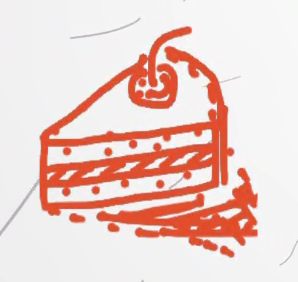
\includegraphics[width=0.3\textwidth]{cake}
	\captionsetup{justification=centering}
	\caption{
		This is not a cake \cite{magritte}, \\
		but a mere simulacrum \cite{beaudrillard}. \\
		$\therefore$ The `cake', as it were, is a lie \cite{rattman}.
	}
	\label{fig:cake}
\end{figure}

When the sunlight strikes raindrops in the air, they act as a prism and form a rainbow. The rainbow is a division of white light into many beautiful colors. These take the shape of a long round arch, with its path high above, and its two ends apparently beyond the horizon. There is , according to legend, a boiling pot of gold at one end. People look, but no one ever finds it. When a man looks for something beyond his reach, his friends say he is looking for the pot of gold at the end of the rainbow.
% Demonstrate wrapping figure
\begin{wrapfigure}{r}{6cm}
	\centering
	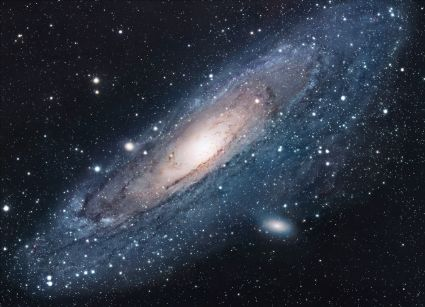
\includegraphics[width=0.8\linewidth]{universe}
	\caption*{\small Claustrophobia vs. Agoraphobia.}
\end{wrapfigure}
Throughout the centuries people have explained the rainbow in various ways. Some have accepted it as a miracle without physical explanation. To the Hebrews it was a token that there would be no more universal floods. The Greeks used to imagine that it was a sign from the gods to foretell war or heavy rain. The Norsemen considered the rainbow as a bridge over which the gods passed from earth to their home in the sky. Others have tried to explain the phenomenon physically. Aristotle thought that the rainbow was caused by reflection of the sun’s rays by the rain. Since then physicists have found that it is not reflection, but refraction by the raindrops which causes the rainbows. Many complicated ideas about the rainbow have been formed. The difference in the rainbow depends considerably upon the size of the drops, and the width of the colored band increases as the size of the drops increases. The actual primary rainbow observed is said to be the effect of super-imposition of a number of bows. If the red of the second bow falls upon the green of the first, the result is to give a bow with an abnormally wide yellow band, since red and green light when mixed form yellow. This is a very common type of bow, one showing mainly red and yellow, with little or no green or blue. % http://www.voxforge.org/home/submitspeech/windows/step-1/dialect/rainbow

% Demonstrate multiple vector figures
\begin{figure}[H]
	\centering
	\begin{subfigure}{0.45\textwidth}
		\centering
		
\includegraphics[width=0.7\textwidth]{potted_plant} 
		\caption{It's a potted plant!}
		\label{fig:potted}
	\end{subfigure}
	\begin{subfigure}{0.45\textwidth}
		\centering
		
\includegraphics[width=0.7\textwidth]{grapes} 
		\caption{It's grapes!}
		\label{fig:grapes}
	\end{subfigure}
	\caption{Caption for a figure with two images.}
	\label{fig:several}
\end{figure}
Vector graphics saved as \texttt{.pdf} can be included as well (which allows us to use emojis \emoji{flushed}).
Several graphics can be bundled in a single figure.
Both of these things can be seen in figure \ref{fig:several} (containing subfigures \ref{fig:potted} and \ref{fig:grapes})

\vfill
The rest of this page would've been blank.
I'd rather have you look at this cute cat, if you don't mind:
\begin{figure}[H]
	\centering
	
\includegraphics[width=\textwidth]{cat-puter}
	\caption{\small this cat \textit{is} quite cute.}
	\label{fig:cat}
\end{figure}
\vfill

\section{Drawing Stuff}

There are several powerful packages (such as \texttt{pgfplots} \ref{sec:pgfplots} and \texttt{tikz} \ref{sec:tikz}) which allow for drawing plots and graphs directly in your \LaTeX{} document.
It be noted how they may noticeably increase compile times. % https://www.overleaf.com/learn/latex/Questions/I_have_a_lot_of_tikz%2C_matlab2tikz_or_pgfplots_figures%2C_so_I%27m_getting_a_compilation_timeout._Can_I_externalise_my_figures%3F

\subsection{With \texttt{pgfplots}}\label{sec:pgfplots}

Some nice graphs can be drawn using the \texttt{pgfplots} package.

% Demonstrate graphing of functions - https://www.overleaf.com/learn/latex/Pgfplots_package
\begin{figure}[H]
	\centering
\begin{tikzpicture}\begin{axis}[
	axis lines = left,
	xlabel = {$x$},
	ylabel = {$f(x)$},
]
%	\addplot[
%		domain=-4:3,
%		samples=100,
%		color=red,
%	]{
%		x^2 - 2*x - 1
%	};
%	\addlegendentry{$x^2 - 2x - 1$}
%	
%	\addplot[
%		domain=-4:3,
%		samples=100,
%		color=blue,
%	]{
%		x^3 / (2^(-x) + 1)
%	};
%	\addlegendentry{$\frac{x^3}{2^{-x} + 1}$}

	\addplot[
		domain=0:1,
		samples=100,
		color=red!25!magenta!40!white,
	]{
		-x^3 + 3*x^2 - 3*x + 1
	};
	\addlegendentry{$-x^3+3x^2-3x+1$}

	\addplot[
		domain=0:1,
		samples=100,
		color=blue!100!cyan!40!white,
	]{
		3*x^3 - 6*x^2 + 3*x
	};
	\addlegendentry{$3x^3 - 6x^2 + 3x$}

	\addplot[
		domain=0:1,
		samples=100,
		color=green!75!teal!40!white,
	]{
		-3*x^3 + 3*x^2
	};
	\addlegendentry{$-3x^3 + 3x^2$}

	\addplot[
		domain=0:1,
		samples=100,
		color=yellow!50!orange!40!white,
	]{
		x^3
	};
	\addlegendentry{$x^3$}
\end{axis}\end{tikzpicture}
	\caption{2D example of Bernstein polynomials.}
	\label{fig:fungraph}
\end{figure}

\begin{figure}[H]
	\centering
\begin{tikzpicture}\begin{axis}[
	hide axis,
	colormap/cool,
]
	\addplot3[
		mesh,
		samples=50,
		domain=-8:8,
	]{
		sin(deg(sqrt(x^2+y^2)))/sqrt(x^2+y^2)
	};
	\addlegendentry{$\frac{\sin(r)}{r}$}
\end{axis}\end{tikzpicture}
	\caption{3D example, using the mesh parameter.}
	\label{fig:meshgraph}
\end{figure}

\subsection{With \texttt{tikz}}\label{sec:tikz}

Here are some graphs drawn using Ti\textit{k}Z.
Doing this can sometimes be a little \emoji{painful} (painfully time-consuming) in my opinion, but the resulting vector graphics are quite timeless.

% Demonstrate drawing of graphs - https://www.baeldung.com/cs/latex-drawing-graphs
\begin{figure}
	\centering
	\begin{tikzpicture}[default/.style={circle, fill=lightgray!33}]
%	\node[rectangle, draw] at (-1,2.5) (mylabel) {$N$ under $f^{++}$};
	\node[default, fill=lightgray!67] at (0,0) (s) {$s$};
	\node[default] at (2,2) (a) {$a$};
	\node[default] at (6,2) (b) {$b$};
	\node[default] at (4,0) (c) {$c$};
	\node[default] at (2,-2) (d) {$d$};
	\node[default] at (6,-2) (e) {$e$};
	\node[default, fill=lightgray!67] at (8,0) (t) {$t$};

	\draw[->] (s) edge node[midway, anchor=south east]{$\textcolor{gray}{8}/8$} (a);
	\draw[->] (s) edge node[midway, anchor=south]{$\textcolor{gray}{8}/8$} (c);
	\draw[->] (s) edge node[midway, anchor=north east]{$\textcolor{gray}{3}/8$} (d);
	\draw[->] (a) edge node[midway, anchor=south]{$\textcolor{gray}{8}/9$} (b);
	\draw[->] (a) edge node[midway, anchor=south west]{$\textcolor{gray}{0}/7$} (c);
	\draw[->] (b) edge node[midway, anchor=south west]{$\textcolor{gray}{12}/13$} (t);
	\draw[->] (c) edge node[midway, anchor=north west]{$\textcolor{gray}{4}/4$} (b);
	\draw[->] (c) edge node[midway, anchor=north west]{$\textcolor{gray}{0}/2$} (d);
	\draw[->] (c) edge node[midway, anchor=south west]{$\textcolor{gray}{4}/12$} (e);
	\draw[->] (d) edge node[midway, anchor=north]{$\textcolor{gray}{3}/6$} (e);
	\draw[->] (e) edge node[midway, anchor=north west]{$\textcolor{gray}{7}/7$} (t);
	\end{tikzpicture}
	\caption{Graph for a flow network $N$.}
	\label{fig:N}
\end{figure}

\begin{figure}
	\centering
	\begin{tikzpicture}[default/.style={circle, fill=lightgray!33}]
%	\node[rectangle, draw] at (-1,2.5) (mylabel) {$N_{f^{++}}$};
	\node[default, fill=lightgray!67] at (0,0) (s) {$s$};
	\node[default] at (2,2) (a) {$a$};
	\node[default] at (6,2) (b) {$b$};
	\node[default] at (4,0) (c) {$c$};
	\node[default] at (2,-2) (d) {$d$};
	\node[default] at (6,-2) (e) {$e$};
	\node[default, fill=lightgray!67] at (8,0) (t) {$t$};
	
	\draw[->] (a) edge[red!50, out=205,in=65,looseness=0.6] node[midway, anchor=south east]{$\textcolor{red}{8}$} (s);
	\draw[->] (c) edge[red!50, out=160,in=20,looseness=0.6] node[midway, anchor=south]{$\textcolor{red}{8}$} (s);
	\draw[->] (s) edge[blue!50, out=295,in=155,looseness=0.6] node[midway, anchor=north east]{$\textcolor{blue}{5}$} (d);
	\draw[->] (d) edge[red!50, out=115,in=335,looseness=0.6] node[midway, anchor=north east]{$\textcolor{red}{3}$} (s);
	\draw[->] (a) edge[blue!50, out=340,in=200,looseness=0.6] node[midway, anchor=south]{$\textcolor{blue}{1}$} (b);
	\draw[->] (b) edge[red!50, out=160,in=20,looseness=0.6] node[midway, anchor=south]{$\textcolor{red}{8}$} (a);
	\draw[->] (a) edge[blue!50, out=295,in=155,looseness=0.6] node[midway, anchor=south west]{$\textcolor{blue}{7}$} (c);
	\draw[->] (b) edge[blue!50, out=295,in=155,looseness=0.6] node[midway, anchor=south west]{$\textcolor{blue}{1}$} (t);
	\draw[->] (t) edge[red!50, out=115,in=335,looseness=0.6] node[midway, anchor=south west]{$\textcolor{red}{12}$} (b);
	\draw[->] (b) edge[red!50, out=205,in=65,looseness=0.6] node[midway, anchor=north west]{$\textcolor{red}{4}$} (c);
	\draw[->] (c) edge[blue!50, out=205,in=65,looseness=0.6] node[midway, anchor=north west]{$\textcolor{blue}{2}$} (d);
	\draw[->] (c) edge[blue!50, out=295,in=155,looseness=0.6] node[midway, anchor=south west]{$\textcolor{blue}{8}$} (e);
	\draw[->] (e) edge[red!50, out=115,in=335,looseness=0.6] node[midway, anchor=south west]{$\textcolor{red}{4}$} (c);
	\draw[->] (d) edge[blue!50, out=340,in=200,looseness=0.6] node[midway, anchor=north]{$\textcolor{blue}{3}$} (e);
	\draw[->] (e) edge[red!50, out=160,in=20,looseness=0.6] node[midway, anchor=north]{$\textcolor{red}{3}$} (d);
	\draw[->] (t) edge[red!50, out=205,in=65,looseness=0.6] node[midway, anchor=north west]{$\textcolor{red}{7}$} (e);
	\end{tikzpicture}
	\caption{Residue graph for the network $N$.}
	\label{fig:Nres}
\end{figure}

\begin{figure}
	\centering
	\begin{tikzpicture}[lbl/.style={circle,fill=pagecol,midway,anchor=center}]
%	\node[rectangle, draw] at (-1,2.5) (mylabel) {$N$ with $(S,T)$};
	\node[circle,fill=cyan!25] at (0,0) (s) {$s$};
	\node[circle,fill=orange!25] at (2,2) (a) {$a$};
	\node[circle,fill=orange!25] at (6,2) (b) {$b$};
	\node[circle,fill=cyan!25] at (4,0) (c) {$c$};
	\node[circle,fill=cyan!25] at (2,-2) (d) {$d$};
	\node[circle,fill=cyan!25] at (6,-2) (e) {$e$};
	\node[circle,fill=orange!25] at (8,0) (t) {$t$};

	\draw[->] (s) edge node[lbl]{$8$} (a);
	\draw[->] (s) edge[lightgray] (c);
	\draw[->] (s) edge[lightgray] (d);
	\draw[->] (a) edge[lightgray] (b);
	\draw[->] (a) edge[lightgray] (c);
	\draw[->] (b) edge[lightgray] (t);
	\draw[->] (c) edge node[lbl]{$4$} (b);
	\draw[->] (c) edge[lightgray] (d);
	\draw[->] (c) edge[lightgray] (e);
	\draw[->] (d) edge[lightgray] (e);
	\draw[->] (e) edge node[lbl]{$7$} (t);
	\end{tikzpicture}
	\caption{An $s$-$t$-cut for network $N$.}
	\label{fig:Ncut}
\end{figure}

\subsection{With \texttt{tcolorbox}}

--- \textit{``These colorboxes are pretty nifty, thanks \href{https://www.ctan.org/pkg/tcolorbox}{Dr.Dr.Sturm!}''}

What follow are some examples with placeholder text inbetween.

\bigskip
% Add an 'algorithm' box
\begin{lalg}{Depth First Search}
	We could implement an iterative version of depth first search as follows
% Typeset some code
% Use custom style defined in preamble
% Optionally specify language syntax highlighting
% Allows escaping math (with this style)
	\begin{lstlisting}[style=L,language=Python]
# The runtime of DFS is in $\On(|V|+|E|)$.
# PRE : `graph` has method `neighbors_of(node)`
def depth_first_search(graph, start_node): 
	stack   = [start_node]
	visited = {start_node}
	while stack:
		current = stack.pop()
		for neighbor in graph.neighbors_of(current):
			if neighbor not in visited:
				stack.append(neighbor)
				visited.add(neighbor)
	\end{lstlisting}
\end{lalg}

\bigskip
\textit{I like this player. It played well. It did not give up.}
\bigskip

% Use a customized tcolorbox - https://xyquadrat.ch/2022/04/04/latex-boxes/
\marginpar{\raggedright Notable thanks to \href{https://xyquadrat.ch/2022/04/04/latex-boxes/}{xyquadrat}}
\begin{tcolorbox}[
	adjusted title=Equivalence Relation, fonttitle=\bfseries,
	boxrule=0mm, leftrule=1mm, arc=0mm, 
	left=1.75mm, toptitle=0.75mm, bottomtitle=0.25mm,
	colframe=brandblue,
	coltitle=textcol, colbacktitle=textcol!10!pagecol,
	coltext=textcol, colback=textcol!5!pagecol,
]
	\def\EAx<#1>{E#1)}
	Given some set $A$ and the relation $\rho\subseteq A\times A$.
	We call $\rho$ an equivalence relation on $A$ if it fulfils the three axioms \EAx<1> - \EAx<3>
% Demonstrate custom enumeration
	\begin{enumerate}[label=\EAx<\arabic*>]
		\item Reflexivity, $\id\subseteq\rho \iff \forall a\in A: a\,\rho\,a$.
		\item Symmetry, $\rho=\hat\rho \iff \forall a,b\in A: a\,\rho\,b \leftrightarrow b\,\rho\,a$.
		\item Transitivity, $\rho^2\subseteq\rho \iff \forall a,b,c\in A: a\,\rho\,b \land b\,\rho\,c \rightarrow a\,\rho\,c$.
	\end{enumerate}
	We call $\rho$ an order relation (or partial order) on $A$ if it fulfils axioms \EAx<1>, \EAx<3> and \EAx<4>.
% 'Continue' enumeration
	\begin{enumerate}[label=\EAx<\arabic*>]\setcounter{enumi}{3}
		\item Antisymmetry, $\rho\cap\hat\rho\subseteq\id \iff \forall a,b\in A: a\,\rho\,b \land b\,\rho\,a \rightarrow b=a$.
	\end{enumerate}
\end{tcolorbox}

\bigskip
\textit{This player dreamed of sunlight and trees. Of fire and water. It dreamed it created. And it dreamed it destroyed. It dreamed it hunted, and was hunted. It dreamed of shelter.}
\bigskip

% Demonstrate tcolorbox with image
\begin{tcolorbox}[
	enhanced,
	adjusted title=\textbf{Binomial Coefficient},
	frame style image=ETH.jpg,
	opacityback=0.80, opacitybacktitle=0.20,
	colback=blue!5!white, colframe=blue!75!black,
]
	The Binomial Coefficient is the coefficient of the $x^k$ term in the polynomial expansion of the binomial power $(1+x)^n$. % % https://en.wikipedia.org/wiki/Binomial_coefficient
	It can be compactly expressed as
	\[ \phantom{1}_nC_k = \prod_{i=1}^k \frac{n+1-i}{i} = \frac{n!}{k!(n-k)!} = \binom{n}{k} \]
	which is usually read as "$n$ choose $k$".
	The coefficient determines the number of ways to choose an unordered subset of $k$ items from a fixed set of $n$ elements.
	It satisfies the recurrence relation $\binom{n}{k} = \binom{n-1}{k-1} + \binom{n-1}{k}$. % https://en.wikipedia.org/wiki/Pascal%27s_triangle
\end{tcolorbox}

\bigskip
\textit{Sometimes the player dreamed it was other things, in other places. Sometimes these dreams were disturbing. Sometimes very beautiful indeed. Sometimes the player woke from one dream into another, then woke from that into a third.}
\bigskip

% Demonstrate tcolorbox with color gradient
\begin{center}\scalebox{1.0}{\begin{tcolorbox}[enhanced,boxrule=0mm,toprule=1.5mm,bottomrule=1.5mm,arc=3mm,arc is angular,rounded corners=all,frame style={left color=red!75!black,right color=red!10!yellow},interior style={white,opacity=0.75},]Let $\angles{M;\,\ast}$ be an algebra with carrier set $M$ and a dyadic operation $\ast$ on $M\times M$. We call $\angles{M;\,\ast}$ a \textit{magma} if it fulfils axiom M1).\begin{enumerate}[label=M\arabic*),leftmargin=15mm]\item$\ast$ satisfies closure, $\forall a,b\in M:a\ast b\in M$.\end{enumerate}\end{tcolorbox}}\end{center} % https://en.wikipedia.org/wiki/Magma_(algebra)

\bigskip
\textit{And the player was a new story, never told before, written in letters of DNA. And the player was a new program, never run before, generated by a sourcecode a billion years old. And the player was a new human, never alive before, made from nothing but milk and love.}
\bigskip

%A \textit{monoid} is an algebra $\angles{M;*,e}$ where\begin{enumerate}[label=M\arabic*)]\item$*$ is associative: $\forall a,b,c\in M:(a*b)*c=a*(b*c)$.\item$e$ is a neutral element: $\forall d\in M:e*d=d*e=d$.\end{enumerate}%https://en.wikipedia.org/wiki/Monoid

% Start appendix sections
\appendix

\section{Random Stuff}

% Manually typeset a chapter quote
\vspace*{-2mm}
{\raggedleft \begin{minipage}{.3\textwidth}
	\footnotesize I never said half the shit people say I did.
	\\\rule{\textwidth}{0.35mm}\\
	\hspace*{\fill}\textit{Albert Einstein}
\end{minipage} \par}
\bigskip

% Line centered on page
\centerline{\mbox{\textsc{Welcome to \uline{this}. where typographical conventions are blasted to smithereens.}}}

% Plaster something over text using manual hacky space commands and also colors
\vspace*{-1.28cm}\hspace*{3.5cm}\scalebox{0.7}{\rotatebox{15}{\fboxrule0.35mm\fcolorbox[HTML]{DFDFDF}{F7F7F7}{\color[HTML]{702FFF}You're just nitpicking and biased, I win, bye bye \raisebox{.25ex}{\scalebox{0.75}{$\heartsuit$}}}}} % https://www.youtube.com/watch?v=sBqk7I5-0I0

\bigskip
\hrule
% Typeset a poem?...
\def\poemline<#1>{{#1}\\}%{\hspace*{1.5cm}{#1}\hspace*{\fill}\\}
\begin{figure}[H]
	\centering
	\sffamily
	\bfseries
	\color{textcol!90!pagecol}
	\poemline<suckity shillity why am i type>%
	\poemline<all of this bullshit that i have to write>%
	\poemline<i could have just copied some text from the web>%
	\poemline<lorem ipsum or whatever it says>%
\end{figure} % https://www.youtube.com/watch?v=1QYxJ69pY0E
\hrule
\bigskip

Recall how under canonical circumstances ($\rightarrow$ cit. \cite{PM10}) equation \big(\ref{eq:conjecture}\big) is believed to be provable from the axioms.
\begin{equation}
	\tag{4.2.1.1}
	\label{eq:conjecture}
	1 + 1 \approx{} 2
\end{equation}
Based.\ on this and making use of some simple re-indexing we have the following trivial result

\normalmarginpar\marginpar{
	\raggedright
	\textcolor{textcol!12.5!pagecol}{...what the \textsl{heeell}} \emoji{Walter}
}
% Demonstrate clusterfuck
\bigskip\resizebox{\textwidth}{!}{\begin{minipage}{2\textwidth}
	\protect{\begin{displaymath}
		\raisebox{0.3ex}{$l\kern-.14em q$}^\bullet(\Lambda)
		= \underbrace{e^{i\pi} + 1} _ {=\ 0}
		- \prod _ {i=0} ^ \infty
		\mleft[
			\operatornamewithlimits{arg\,ker} _ {
				\substack{
					r\in\R^\times \\
					\nexists n\,:\,r=F_n
				}
			}
			\bigcup _ {\ell\in\Lambda}
			\left\{
				\ell\circ\varphi_0\in\mathcal{C}^\infty
			\;\middle\vert\;
				\varphi_0
				\triangleq
				\operatornamewithlimits{
					\emoji{trollface}%\raisebox{-.8ex}{\includegraphics[height=16pt]{trollQ}}
				} _ {k=1} ^ {\infty}
				\zeta^{(r)}(k!!)
				\land
				\mleft(
					\liminf _ {\chi\to 0^-} \varphi_0(\chi) \notin\mathbb{Q}_{\geq0}
					\lor
					\mleft(
						\forall p\neq q :
							p \equiv_{251} \ceil{(\ell\cdot\digamma)(q)}
							\rightarrow
							\operatorname{supp}(\partial\varphi_0)=\varnothing
					\mright)
				\mright)
			\right\}
		\mright]
		+ \mleft.\frac{7\sqrt[\varepsilon]{\pi}}{12}\mright|^{\varepsilon=\sqrt2}
	\end{displaymath}}
\end{minipage}}

\bigskip
% Demonstrate unbreakable paragraphs - https://texfaq.org/FAQ-nopagebrk
\needspace{2\baselineskip}
\textit{\large\guillemotleft What are some of the “ugliest” parts of math?\guillemotright}
% Demonstrate list of descriptions with nice indents
\begin{description}[nosep,noitemsep,leftmargin=5mm]
	\item[Point-set topology.] Too many pathologies. Nowadays the only topologies for me are Grothendieck topologies.
	\item[Weights, in the context of Lie algebras.] The constructions are high\-ly non-ca\-no\-ni\-cal if not even arbitrary sometimes.
	\item[Elementary topoi.] Unless you're a logician, I can't see why you would prefer them to honest-to-Grothendieck sheaf topoi (feel free to change my mind).
	\item[Classical algebraic geometry à la Weil.] It was a mess (again, due to point-set topology being a pain), and not to mention very restrictive, as varieties only behave well over algebraically closed fields.
	\item[Topological vector spaces.] They are not ugly per se, but extremely delicate and subtle, and daing with them can sometimes involve hours if not days trying to find the right norm on a perfectly fine algebraic object (e.g. tensor products of Banach spaces).
	\item[Tate's rigid analytic varieties and Berkovich spaces.] They are practical and easy to visualise, but better to have a nice category with bad objects than a bad category of nice objects. One also needs to impose all sorts of extra finiteness conditions on them in order to be able to even begin computing their cohomologies. Luckily, these categories embed into the category of adic spaces (in the sense of Huber), which is much nicer, especially if you were to restrict down to the subcategory of perfectoid spaces.
\end{description}
% Demonstrate overlapping of symbols - https://tex.stackexchange.com/questions/620022/overlay-symbols-via-ooalign
(\^{} What the heck is \href{https://www.reddit.com/r/math/comments/rud9uq/comment/hr1mdli}{this} guy talking about) % https://www.reddit.com/r/math/comments/rud9uq/comment/hr1mdli

% Add frame directly onto content
%\frame{
%	\resizebox{0.95\textwidth}{!}{
%		The phrase "it's just a game" is such a weak mindset. You are ok with what happened, losing, imperfection of a craft. When you stop getting angry after losing, you've lost twice.
%	}
%}

%\bigskip
%\hrule
%\centerline{\resizebox{\textwidth}{!}{$\neg\exists x : \forall y : (P(y,x) \leftrightarrow \neg P(y,y))$}}
%\hrule

\newpage
\hfill$\underset{\textit{so below}}{\textit{as above}}$

\needspace{2\baselineskip}
\textit{\textbf{``What's your Sauce Code?''}}
\begingroup
	\makeatletter
		\DeclareRobustCommand\ttfamily{
			\not@math@alphabet\ttfamily\mathtt
			\fontfamily\ttdefault\footnotesize\selectfont
		}
	\makeatother % https://tex.stackexchange.com/questions/158778/all-ttfamily-font-change-font-size#158779
	\color{-pagecol}
% Demonstrate some unformatted code
\begin{listing}{1}
double a[4][4];
double b[4][4];
double c[4][4]; // set to zero
/* Multiply 4 x 4 matrices a and b */
void mmm(double *a, double *b, double *c, int n) {
  int i, j, k;
  for (i = 0; i < 4; i++)
    for (j = 0; j < 4; j++)
      for (k = 0; k < 4; k++)
        c[i*4+j] += a[i*4 + k]*b[k*4 + j];
}
// At this point, I'd like to take a moment to speak to you about the Adobe PSD
// format. PSD is not a good format. PSD is not even a bad format. Calling it
// such would be an insult to other bad formats, such as PCX or JPEG. No, PSD
// is an abysmal format. Having worked on this code for several weeks now, my
// hate for PSD has grown to a raging fire that burns with the fierce passion
// of a million suns.
//
// If there are two different ways of doing something, PSD will do both, in
// different places. It will then make up three more ways no sane human would
// think of, and do those too. PSD makes inconsistency an art form. Why, for
// instance, did it suddenly decide that *these* particular chunks should be
// aligned to four bytes, and that this alignement should *not* be included in
// the size? Other chunks in other places are either unaligned, or aligned with
// the alignment included in the size. Here, though, it is not included. Either
// one of these three behaviours would be fine. A sane format would pick one.
// PSD, of course, uses all three, and more.
//
// Trying to get data out of a PSD file is like trying to find something in the
// attic of your eccentric old uncle who died in a freak freshwater shark
// attack on his 58th birthday. That last detail may not be important for the
// purposes of the simile, but at this point I am spending a lot of time
// imagining amusing fates for the people responsible for this Rube Goldberg of
// a file format.
//
// Earlier, I tried to get a hold of the latest specs for the PSD file format.
// To do this, I had to apply to them for permission to apply to them to have
// them consider sending me this sacred tome. This would have involved faxing
// them a copy of some document or other, probably signed in blood. I can only
// imagine that they make this process so difficult because they are intensely
// ashamed of having created this abomination. I was naturally not gullible
// enough to go through with this procedure, but if I had done so, I would have
// printed out every single page of the spec, and set them all on fire. Were it
// within my power, I would gather every single copy of those specs, and launch
// them on a spaceship directly into the sun.
//
// PSD is not my favourite file format.\end{listing}
\endgroup % https://github.com/gco/xee/blob/master/XeePhotoshopLoader.m#L108-L136

\vfill\hfill$\underset{\textit{so above}}{\textit{as below}}$

%\clearpage
%\vspace*{\fill}
%\begin{figure}[H]
%	\raggedleft
%	\textit{\large ``In this world, is the destiny of mankind controlled by some transcendental entity or law? Is it like the hand of God hovering above? At least it is true that man has no control, even over his own will. Man takes up the sword in order to shield the small wound in his heart sustained in a far-off time beyond remembrance. Man wields the sword so that he may die smiling in some far-off time beyond perception.''}
%\end{figure}
%\vspace*{\fill}
%\clearpage

\clearpage
	\pagecolor{pergament}
	\color{sepia}
	\begin{multicols}{2}
% Demonstrate input file
	\raisebox{-0.4ex}{\huge V}\resizebox{0pt}{0pt}{on\space Franz\space Kafka\space -\space v}or dem Gesetz steht ein Türhüter. Zu diesem Türhüter kommt ein Mann vom Lande und bittet um Eintritt in das Gesetz. Aber der Türhüter sagt, dass er ihm jetzt den Eintritt nicht gewähren könne. Der Mann überlegt und fragt dann, ob er also später werde eintreten dürfen. „Es ist möglich,“ sagt der Türhüter, „jetzt aber nicht.“ Da das Tor zum Gesetz offen steht wie immer und der Türhüter beiseite tritt, bückt sich der Mann, um durch das Tor in das Innere zu sehen. Als der Türhüter das merkt, lacht er und sagt: „Wenn es dich so lockt, versuche es doch trotz meines Verbotes hineinzugehen. Merke aber: Ich bin mächtig. Und ich bin nur der unterste Türhüter. Von Saal zu Saal stehen aber Türhüter, einer mächtiger als der andere. Schon den Anblick des Dritten kann nicht einmal ich mehr ertragen.“ Solche Schwierigkeiten hat der Mann vom Lande nicht erwartet; das Gesetz soll doch jedem und immer zugänglich sein, denkt er, aber als er jetzt den Türhüter in seinem Pelzmantel genauer ansieht, seine grosse Spitznase, den langen, dünnen, schwarzen tartarischen Bart, entschliesst er sich doch lieber zu warten, bis er die Erlaubnis zum Eintritt bekommt. Der Türhüter gibt ihm einen Schemel und lässt ihn seitwärts von der Tür sich niedersetzen. Dort sitzt er Tage und Jahre. Er macht viele Versuche eingelassen zu werden und ermüdet den Türhüter durch seine Bitten. Der Türhüter stellt öfters kleine Verhöre mit ihm an, fragt ihn über seine Heimat aus und nach vielem andern, es sind aber teilnahmslose Fragen, wie sie grosse Herren stellen, und zum Schlusse sagt er ihm immer wieder, dass er ihn noch nicht einlassen könne. Der Mann, der sich für seine Reise mit vielem ausgerüstet hat, verwendet alles, und sei es noch so wertvoll, um den Türhüter zu bestechen. Dieser nimmt zwar alles an, aber sagt dabei: „Ich nehme es nur an, damit du nicht glaubst, etwas versäumt zu haben.“ Während der vielen Jahre beobachtet der Mann den Türhüter fast ununterbrochen. Er vergisst die andern Türhüter und dieser erste scheint ihm das einzige Hindernis für den Eintritt in das Gesetz. Er verflucht den unglücklichen Zufall, in den ersten Jahren rücksichtslos und laut, später als er alt wird, brummt er nur noch vor sich hin. Er wird kindisch und da er in dem jahrelangen Studium des Türhüters auch die Flöhe in seinem Pelzkragen erkannt hat, bittet er auch die Flöhe ihm zu helfen und den Türhüter umzustimmen. Schliesslich wird sein Augenlicht schwach und er weiss nicht, ob es um ihn wirklich dunkler wird oder ob ihn nur seine Augen täuschen. Wohl aber erkennt er jetzt im Dunkel einen Glanz, der unverlöschlich aus der Türe des Gesetzes bricht. Nun lebt er nicht mehr lange. Vor seinem Tode sammeln sich in seinem Kopfe alle Erfahrungen der ganzen Zeit zu einer Frage, die er bisher an den Türhüter noch nicht gestellt hat. Er winkt ihm zu, da er seinen erstarrenden Körper nicht mehr aufrichten kann. Der Türhüter muss sich tief zu ihm hinunterneigen, denn der Grössenunterschied hat sich sehr zu ungunsten des Mannes verändert. „Was willst du denn jetzt noch wissen?“ fragt der Türhüter, „du bist unersättlich.“ „Alle streben doch nach dem Gesetz,“ sagt der Mann, „wieso kommt es, dass in den vielen Jahren niemand ausser mir Einlass verlangt hat?“ Der Türhüter erkennt, dass der Mann schon an seinem Ende ist und, um sein vergehendes Gehör noch zu erreichen, brüllt er ihn an: „Hier konnte niemand sonst Einlass erhalten, denn dieser Eingang war nur für dich bestimmt. Ich gehe jetzt und schliesse ihn.“

	\end{multicols}
	\fancypagestyle{gesetzstyle}{
		\fancyhf{} \renewcommand{\headrulewidth}{0pt}
		\fancyhead[C]{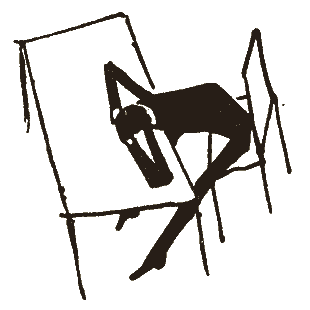
\includegraphics[height=20pt]{kafka}}
	}\thispagestyle{gesetzstyle}
	\color{textcol}
	\afterpage{\nopagecolor}
\clearpage


%\usepackage[latin1]{inputenc} % breaks nothing but is useless - https://tex.stackexchange.com/questions/44694/fontenc-vs-inputenc
%\usepackage{fontspec} % Wtf - https://www.overleaf.com/learn/latex/Questions/I_have_a_custom_font_I%27d_like_to_load_to_my_document._How_can_I_do_this%3F#If_you.27re_using_XeLaTeX_or_LuaLaTeX
%\usepackage{luatextra}\defaultfontfeatures{Ligatures=TeX} % What??? - https://tex.stackexchange.com/questions/641889/german-umlauts-are-ok-but-%C3%9F-appears-as-ss

%\begin{flushright}
%	Using \texttt{biblatex} you can display a bibliography divided into sections, depending on citation type. 
%	Let's cite! Einstein's journal paper \cite{einstein} and Dirac's book \cite{dirac} are physics-related items. 
%	Next, \textit{The \LaTeX\ Companion} book \cite{latexcompanion}, Donald Knuth's website \cite{knuthwebsite}, \textit{The Comprehensive Tex Archive Network} (CTAN) \cite{ctan} are \LaTeX-related items; but the others, Donald Knuth's items, \cite{knuth-fa,knuth-acp} are dedicated to programming.
%\end{flushright}
% Generate bibliography using biblatex
%\printbibliography[heading=bibintoc] % https://www.overleaf.com/learn/latex/Bibliography_management_in_LaTeX

%\begin{flushright}
%	``I always thought something was fundamentally wrong with the universe'' \citep{adams1995hitchhiker}
%\end{flushright}
%% Generate bibliography using natbib - https://www.overleaf.com/learn/latex/Bibliography_management_with_natbib
%\bibliography{references}

% Generate bibliography .. - https://www.overleaf.com/learn/latex/Bibliography_management_with_bibtex
\begin{thebibliography}{9}
	\bibitem{texbook}
		Donald E. Knuth (1986) \emph{The \TeX{} Book}, Addison-Wesley Professional.
	\bibitem{lamport94}
		Leslie Lamport (1994) \emph{\LaTeX: a document preparation system}, Addison Wesley, Massachusetts, 2nd ed.
	\bibitem{PM10}
		Alfred North Whitehead and Bertrand Russel (1910) \emph{Principia Mathematica}, Cambridge at the University Press.
	\bibitem{magritte}
		\url{https://en.wikipedia.org/wiki/The_Treachery_of_Images}
	\bibitem{beaudrillard}
		\url{https://en.wikipedia.org/wiki/Simulacra_and_Simulation}
	\bibitem{rattman}
		\url{https://en.wikipedia.org/wiki/The_cake_is_a_lie}
\end{thebibliography}

% Generate list of figures
\listoffigures
% Generate list of tables
\listoftables

% End
\newpage
\phantom{hello, world}
\fancypagestyle{endstyle}{
	\fancyhf{} \renewcommand{\headrulewidth}{0pt}
	%\fancyhead[C]{\textit{This page intentionally left blank(?)}}
	\fancyfoot[C]{\color{textcol!50!pagecol}\textit{``Falls du Schreibfehler findest, darfst du diese selbstverständlich gerne behalten.''}} % https://bertimo.jimdofree.com/
}\thispagestyle{endstyle}

% ~:------------------------------------+------------------------------------:~

                                   \end{document}

% ~:------------------------------------+------------------------------------:~